\chapter{Gravitational decoherence at the quantum level}\label{ch:gravdec}

\section{Di\'osi--Penrose}

Di\'osi~\cite{Diosi1987,Diosi1989} and Penrose~\cite{Penrose1996} proposed that a superposition
of two mass distributions separated by more than their size decays on the timescale
\begin{equation}
 \tau_{\mathrm{DP}}\simeq\frac{\hbar}{E_G},\qquad E_G\simeq\frac{Gm^2}{R},
\end{equation}
with $E_G$ the gravitational self-energy of the difference of the mass distributions. The
prediction is temperature-independent. For one class of mass distributions it has been
constrained by underground radiation measurements~\cite{Donadi2021}. Levitated
optomechanics is approaching the regime needed to test it directly~\cite{RomeroIsart2011,Gonzalez2021}.

\section{The IAM rate}

IAM gives a different law. It takes the information production rate to be
\begin{equation}
 \frac{dN_{\mathrm{bits}}}{dt}=\frac{E_G^2}{\hbar\,\kB T\ln2},
\end{equation}
and the boundary capacity of the superposition is $S_{\mathrm{boundary}}=\kB T/E_G$. Both are postulated, not derived from the law. \conjecture{} The temperature dependence that follows runs opposite to every
known environmental decoherence, which strengthens with temperature; that is what makes it testable.
Integrating $\Gamma_{\mathrm{info}}/S_{\mathrm{boundary}}$ gives
\begin{equation}
 \ln E_q(t)=\frac{E_G^3}{\hbar\,\kB^2T^2\ln2}\,t,\qquad
 \boxed{\;\tau_{\mathrm{IAM}}=\frac{\hbar\,\kB^2T^2\ln2}{E_G^3}\;}
 \label{eq:tauIAM}
\end{equation}
This is a plain exponential decay with time constant $\tau_{\mathrm{IAM}}$. \calc{} An alternative carries over the functional form of the
cosmic activation function. It does not follow from the integral above and is an assumption: \conjecture
\begin{equation}
 C_{\mathrm{IAM}}(t)=1-\frac{E_q(t/\tau_{\mathrm{IAM}})}{e},\qquad E_q(\eta)=\exp(1-1/\eta),
\end{equation}
in place of the exponential $C_{\mathrm{DP}}=\exp(-t/\tau_{\mathrm{DP}})$. The corresponding
Lindblad generator~\cite{Lindblad1976} is $d\rho/d\eta=\Gamma(\eta)\,[L\rho L^\dagger-\tfrac12\{L^\dagger L,\rho\}]$
with $L\propto\hat x$ and $\Gamma(\eta)=\eta^{-2}e^{1-1/\eta}$.

\section{Signatures}

\begin{figure}[htbp]\centering
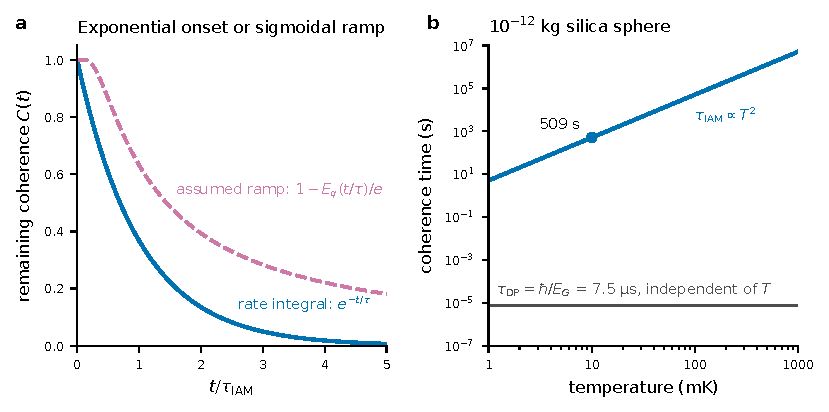
\includegraphics[width=\textwidth]{figures/part5/fig_decoherence_profiles.pdf}
\caption{(a) Remaining coherence against $t/\tau_{\rm IAM}$: the plain exponential the rate integral gives, and the ramp $1-E_q(t/\tau)/e$, $E_q(\eta)=\exp(1-1/\eta)$, carried over from the cosmology \conjecture. (b) $\tau_{\rm IAM}$ against temperature for a $10^{-12}$\,kg silica sphere ($\rho=2200$\,kg\,m$^{-3}$, $R=4.8\,\mu$m, $E_G=1.4\times10^{-29}$\,J): 509\,s at 10\,mK, growing as $T^2$ (factors 4 and 16 at 20 and 40\,mK), against the temperature-independent $\tau_{\rm DP}=7.5\,\mu$s. \prediction}\label{fig:decoherence_profiles}
\end{figure}

The IAM law differs from Di\'osi--Penrose in three ways, each testable:
\begin{enumerate}
 \item \textbf{Temperature.} $\tau_{\mathrm{IAM}}\propto T^2$: a \emph{hotter} object stays
       coherent \emph{longer}. The Di\'osi--Penrose time is independent of $T$. Running at 10,
       20 and 40~mK should lengthen $\tau$ by factors of 4 and 16.
 \item \textbf{Mass.} $\tau_{\mathrm{IAM}}\propto E_G^{-3}\propto m^{-6}R^3$, against
       $\tau_{\mathrm{DP}}\propto m^{-2}R$ (at fixed density, $\tau_{\mathrm{IAM}}\propto m^{-5}$ and $\tau_{\mathrm{DP}}\propto m^{-5/3}$).
 \item \textbf{Profile (only if the assumed ramp holds).} $C(t)$ would have zero slope at $t=0$ and a sigmoidal onset; the rate integral
       gives an exponential. A measured exponential onset with the $T^2$ and mass scalings would support the rate and reject the ramp.
\end{enumerate}

\begin{checkbox}[title={Independent check: the numbers}]
\textbf{Dimensions.} $\hbar\kB^2T^2/E_G^3$ has units $\mathrm{J\,s}\cdot\mathrm{J}^2/\mathrm{J}^3=\mathrm s$.
Correct.

\textbf{The cat.} $m=4$~kg, $E_G=7.1\times10^{-9}$~J (implying $R\approx0.15$~m), $T=300$~K:
Eq.~\eqref{eq:tauIAM} gives $3.5\times10^{-51}$~s. \calc{} Environmental decoherence of a warm macroscopic body is faster still, so the number illustrates the formula; it is not the
mechanism that makes a cat classical.

\textbf{The nanosphere.} For a $10^{-12}$~kg silica sphere ($\rho=2200\ \mathrm{kg\,m^{-3}}$,
$R=4.8\ \mu$m), $E_G=1.4\times10^{-29}$~J, and Eq.~\eqref{eq:tauIAM} gives $\tau_{\mathrm{IAM}}=509$~s
at 10~mK, against $\tau_{\mathrm{DP}}=7.5\ \mu$s. \calc{} At physical densities the IAM time for a
$10^{-12}$~kg sphere is about $7\times10^{7}$ times the Di\'osi--Penrose time, so the two models are
distinguished by \emph{which one is seen at all}, not by their profile shapes.
\end{checkbox}

\section{Where the two sectors meet}

In the dual-sector picture, the matter sector ($\mu<1$) decoheres gravitationally and the
photon sector ($\Sigma=1$) does not. \conjecture Trapped ions ($m\sim10^{-25}$~kg) and superconducting
qubits (effective moving mass $\sim10^{-20}$~kg) have $\tau_{\mathrm{IAM}}$ and
$\tau_{\mathrm{DP}}$ both far beyond any practical time. Gravitational decoherence is
irrelevant to current quantum computers under either model. Their decoherence is
electromagnetic and material, which is where Part~\ref{part:3} reads them.
